\documentclass{standalone}
\usepackage{tikz}
\usepackage{xcolor}
\definecolor{forestgreen}{RGB}{34,139,34}

\begin{document}
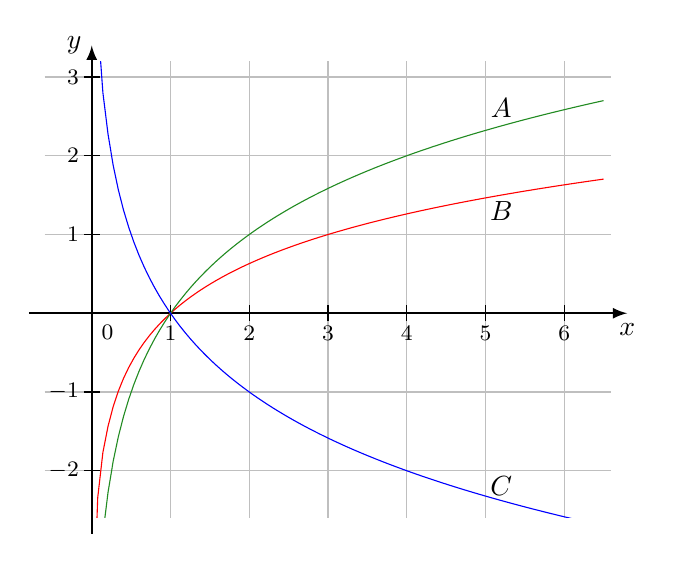
\begin{tikzpicture}[cross/.style={draw, cross out, minimum size=2*(#1-1pt), inner sep=0pt, outer sep=0pt}, x=10mm, y=10mm, 
    >=latex,   %Voreinstellung für Pfeilspitzen
    font= \footnotesize, scale=1]
    %Raster zeichnen
    \draw [color=gray!50]  [step=10mm] (-0.6,-2.6) grid (6.6,3.2);
    % Achsen zeichnen
    \draw[->,thick] (-0.8,0) -- (6.8,0) node[right, below] {\normalsize $x$};
    \draw[->,thick] (0,-2.8) -- (0,3.4) node[above, left] {\normalsize $y$};
    % Achsen beschriften
    \foreach \x in {1,2,...,6} \draw (\x,-.1) -- (\x,.1) node[below=4pt] {$\x$};
    \foreach \y in {-2,-1,1,2,3} \draw (-.1,\y) -- (.1,\y) node[left=4pt] {$\y$};
    % Besserer Ursprung
    \draw[color=black] (0pt,-7pt) node[right] {$0$};
    %Funktionen zeichnen:
    \clip(-0.6,-2.6) rectangle (6.6,3.2); %Bildbereich
    \draw[red,domain=0.01:6.5,samples=100] plot (\x, {ln(\x)/ln(3)});
    \draw[forestgreen,domain=0.01:6.5,samples=100] plot (\x, {ln(\x)/ln(2)});
    \draw[blue,domain=0.01:6.5,samples=100] plot (\x, {ln(\x)/ln(0.5)});
    %Beschriftung
    \node[black]  at (5.2,2.6) {\normalsize$A$};
    \node[black]  at (5.2,1.3) {\normalsize$B$};
    \node[black]  at (5.2,-2.2) {\normalsize$C$};
\end{tikzpicture}


\end{document}